\section{Project Dependent Preparations}
\label{sec:pdp}
\subsection{Software and Simulation Environment}

Upskilling has been undertaken across the full software system required for this project. The simulation environment is built on ROS~2 Humble and Gazebo Ignition, with inter-process communication handled via the \texttt{ros\_gz\_bridge}. A motion capture emulator replicates the system that will be used in physical experiments, publishing pose and velocity estimates at 120\,Hz over the \texttt{/drone\_N/motion\_capture\_state} topic. Low-level flight control is handled by Betaflight software, interfaced via an ExpressLRS (ELRS) command bridge that accepts roll, pitch, throttle, and yaw channels.

\subsection{Multi-Drone Control Architecture}

A coordinated multi-drone control architecture has been designed. The system consists of a centralised \textit{Central Controller} node and four independent \textit{Controller MPC} nodes, one per drone. The Central Controller owns the master trajectory clock and broadcasts a synchronised step index over the \texttt{/fleet/step} topic at 30\,Hz. Each controller shadows this step index and evaluates its MPC against a drone-specific trajectory that incorporates a fixed spatial offset corresponding to the desired formation geometry. This design ensures all drones track the same point in the trajectory simultaneously without requiring inter-drone communication or a shared state estimate.

\subsection{Preliminary Simulation Results}

The coordinated flight system has been validated in Gazebo. Figure~\ref{fig:formation_trajectories} shows the recorded trajectories of all four drones during a complete flight sequence, circle markers indicate start positions and cross markers indicate end positions. The formation is maintained throughout the circle phase, with each drone tracking a circle trajectory. A recording of the simulation is available at \url{https://www.youtube.com/watch?v=I-RICF6KPtc}.

\begin{figure}[h]
    \centering
    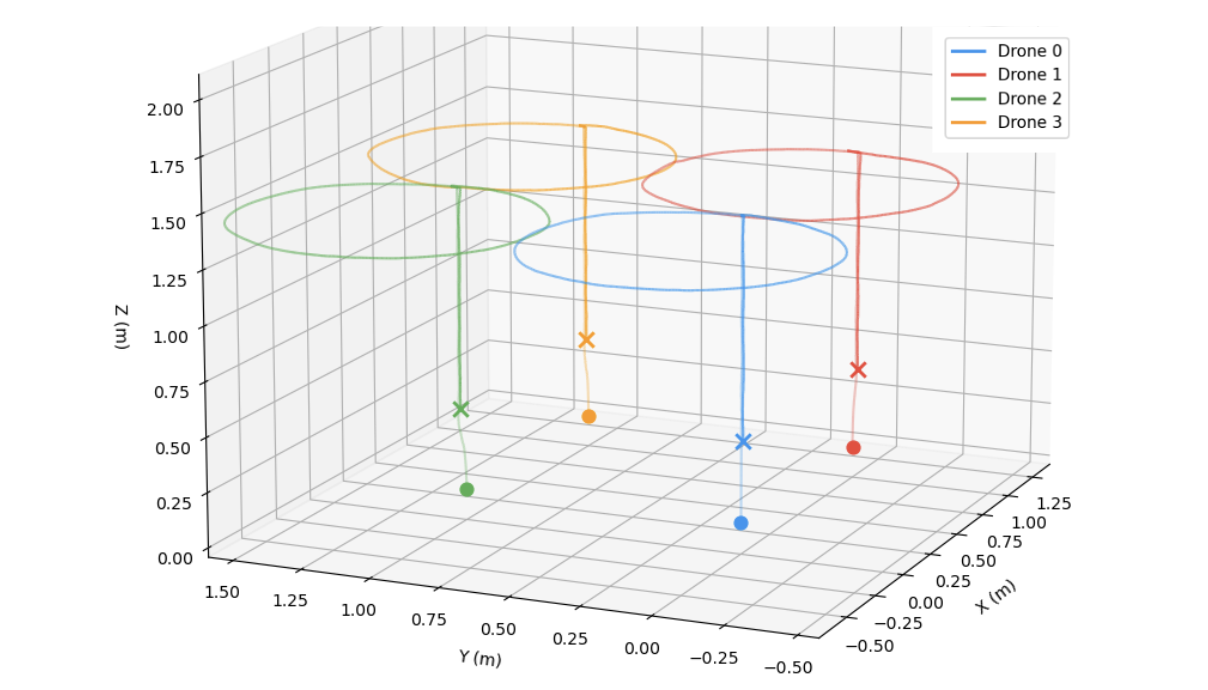
\includegraphics[width=0.85\textwidth]{Images/Screenshot 2026-04-20 at 11.35.37 AM.png}
    \caption{3D view of the four drone formation trajectories during a flight sequence.}
    \label{fig:formation_trajectories}
\end{figure}

Formation tracking performance was quantified by finding the deviation of each drone from its expected offset relative to Drone~0's actual position at each timestep. The results are summarised in Table~\ref{tab:formation_error} and plotted over time in Figure~\ref{fig:formation_error}.

\begin{table}[h]
    \centering
    \caption{Formation tracking error relative to Drone 0 during the circle trajectory phase.}
    \label{tab:formation_error}
    \begin{tabular}{lccc}
        \hline
        \textbf{Drone} & \textbf{Mean Error (m)} & \textbf{Max Error (m)} & \textbf{RMS Error (m)} \\
        \hline
        Drone 1 & 0.0220 & 0.0487 & 0.0249 \\
        Drone 2 & 0.0234 & 0.0537 & 0.0264 \\
        Drone 3 & 0.0311 & 0.0690 & 0.0347 \\
        \hline
    \end{tabular}
\end{table}

\begin{figure}[h]
    \centering
    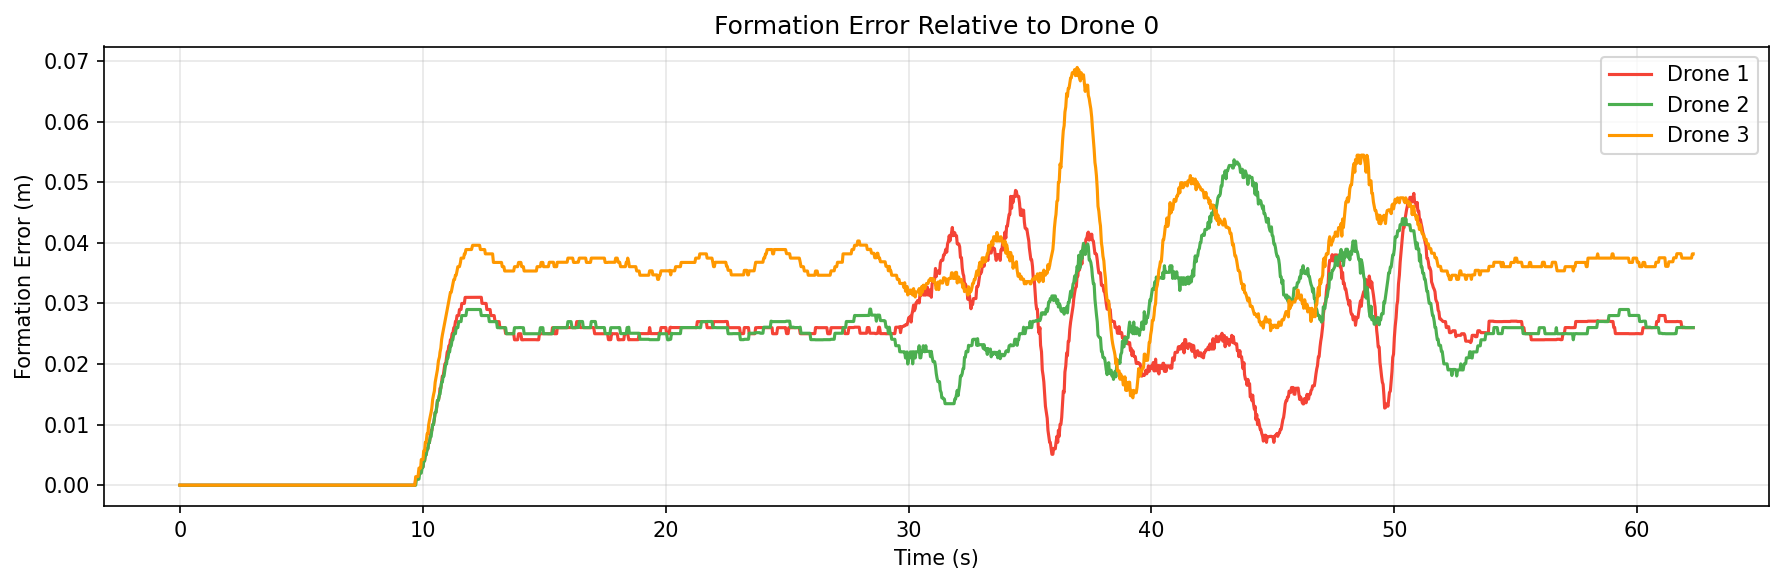
\includegraphics[width=1\textwidth]{Images/formation_error.png}
    \caption{Formation error over time for Drones 1--3 relative to Drone~0.}
    \label{fig:formation_error}
\end{figure}

All three follower drones maintain under 5\,cm mean formation error, with RMS errors below 3.5\,cm. Drone~3, located at the $(1,1)$ offset position, exhibits the largest error, which is consistent with its greater distance from the formation reference drone and the compounding of any synchronisation delay across both axes. These results demonstrate that the architecture achieves tight formation coordination in the current simulation. \\

An additional Gazebo world has been constructed in which all four drones are tethered to a payload (Figure~\ref{fig:world_cables}). The cable model is based on the gazebo model in \cite{grahamDevelopmentQuadrotorSlung}. This will serve as the main testing environment for cooperative load carrying. The tether geometry and payload mass properties have been configured, and the simulation is operational. Controller development for the tethered case will proceed in the next phase.

\begin{figure}[h]
    \centering
    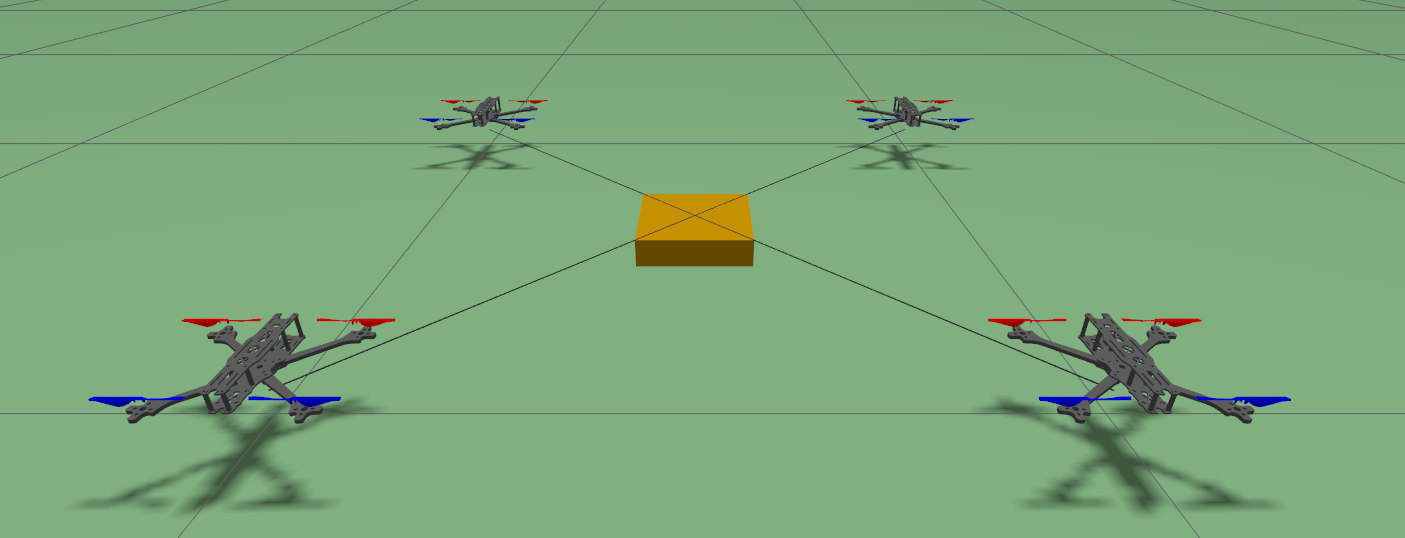
\includegraphics[width=0.8\textwidth]{Images/world_cables.png}
    \caption{Gazebo world with tethered payload.}
    \label{fig:world_cables}
\end{figure}